\begin{parag}{Cover's theorem}
	\begin{theoreme}[Cover's theorem]
    A complex pattern-classification problem, cast in a high-dimensional space nonlinearly, is more likely to be linearly separable than in a low-dimensional space, provided that the space is not densely populated.
    \end{theoreme}
\end{parag}

\section{Overfitting, Cross-validation and Regularization}
The goal of this section is to understand the notions of model complexity and overfitting. We will introduce several strategies to select a model that does not overfit and introduce the notion of regularization to prevent overfitting.

\begin{parag}{Model complexity}
    As we have moved from linear models to nonlinear ones, we have obtained increasing flexibility:
	\begin{itemize}
	    \item We do not longer assume that the ouput linearly depends on the input
	    \item We can handle classification problems in which the classes are nonlinearly separable
	\end{itemize}
	This flexibility, however, may sometimes make the model too complex for the task at hand. 
	To illustrate this let us look at an example with k-NN:
\end{parag}
\begin{parag}{Example}
	Using k-NN and some data for instance:\\
	put images\\
	The number of neighbors $k$ influences a lot of our algorithm react for instance let us take some examples of values for $k$:\\
	put another image here (both)o\\
	As you can see by adding/removing $k$ our algorithm our model differs. The question we are trying to answer is, what $k$ is the best and first, what a low $k$ do, what a high $k$ do?
\end{parag}
\begin{parag}{k-NN: Training vs test}
    Let's look at typical training and test curves (from T. Srivastava @ AnalyticsVidhya)
	\begin{center}
	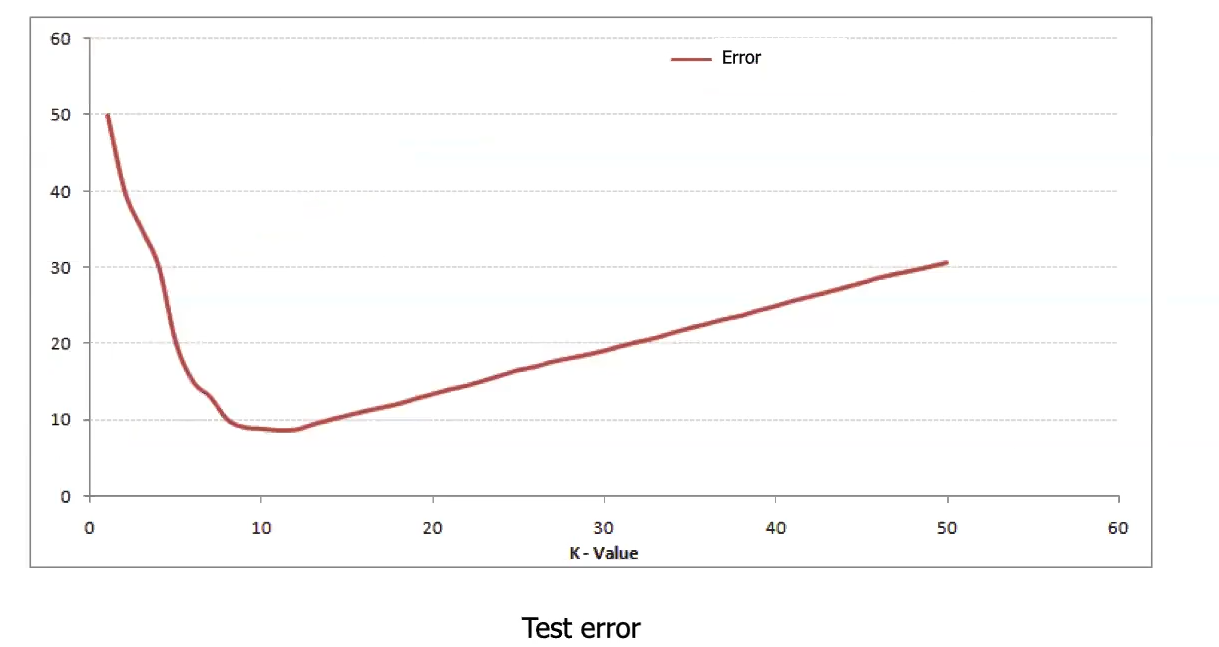
\includegraphics[scale=0.3]{screenshots/2026-03-11.png}
	\end{center}
	As we can see when having low $k$ we are \important{overfitting}, meaning that copied our training data, but on on test data, the error will be high. And after passing $10$ what we observed is that our model is actually performing worse than before even though we are incrementing $k$; our model is \important{underfitting}. In this case the error is large on both the training data and the test data. This is called \important{underfitting}.
	\begin{subparag}{Remark}
	    Tis behavior is \important{not} specific to k-NN. It can happen in most machine learning algorithm.
	\end{subparag}
\end{parag}
\begin{framedremark}
I find the example quite misleading. Here we see a low $k$ as the overfitting case. As if the model is to easy then we are overfitting. But in general and as we will see later, the easier the model the more underfitting our model is doing. And it also works the other way around, the more our model is complex, the more our model is overfitting.
\end{framedremark}


\begin{parag}{Overfitting vs Underfitting}
	Those are general phenomenons. And we can often links the error/fitting to the model complexity. By increasing the complexity we are also more prone to have better results on our training data, maybe too much which we will lead us to have a model that is overfitting.
    \begin{center}
    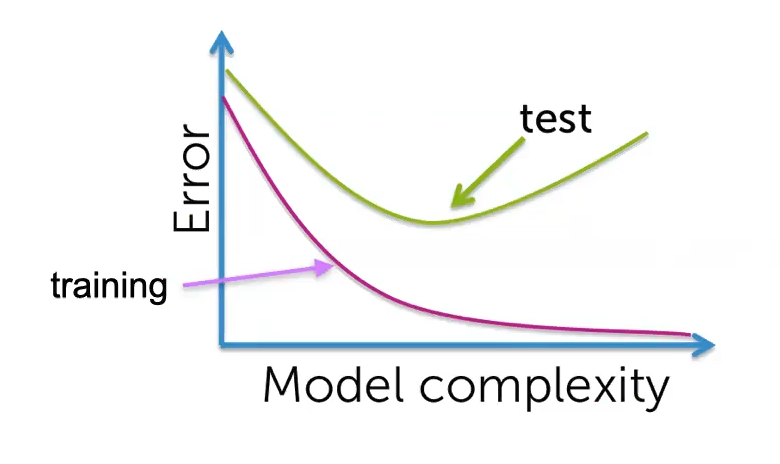
\includegraphics[scale=0.3]{screenshots/2026-03-11_1.png}
    \end{center}
\end{parag}

\begin{parag}{Model Selection}

	The question is then:
	\begin{center}
	    Since we don't have access to the test data,  how do we choose the right complexity for the model?
	\end{center}
	Our solution is is \important{Cross-validation}
	\begin{subparag}{Remark}
	    The following material was adapted from Andrew Moore's cross-validation slides
	\end{subparag}
\end{parag}


\begin{parag}{Cross-validation: Toy example}
	Let us have a regression problem with a 1D input $x$ and a 1D output $y$. We are given the following training observations:
	\begin{center}
	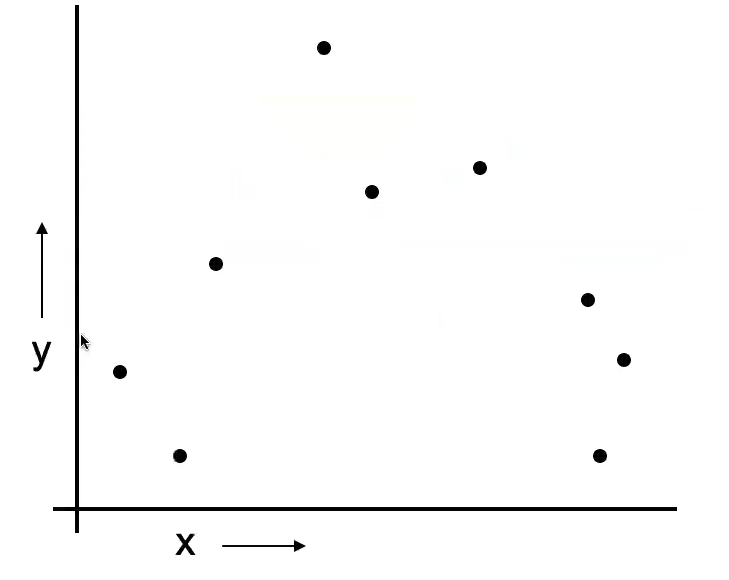
\includegraphics[scale=0.2]{screenshots/2026-03-11_2.png}
	\end{center}
	We will consider 3 different models (of increasing complexity):
	\begin{center}
	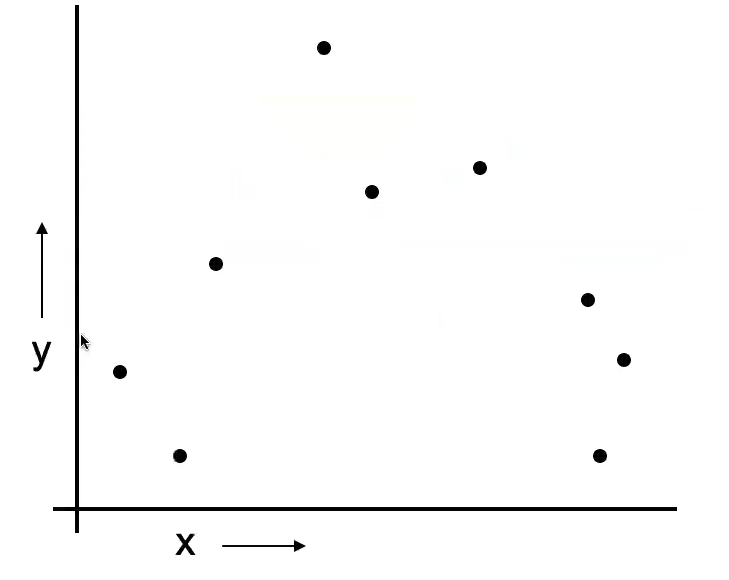
\includegraphics[scale=0.2]{screenshots/2026-03-11_2.png}
	\end{center}
	As our goal is to fit our data, why don't choose the one that best fits the data?\\
	$ $\\
	What we truly care about is how well the model is going to predict future data drawn from the same distribution. To do so, why not simulate data based on our training data.
\end{parag}
\begin{parag}{Validation set method}
	We take our training data which we will split into two parts, one as the \important{training set}, and the other as a \important{validation set} (e.g., 30\% of the data). 
    \begin{center}
    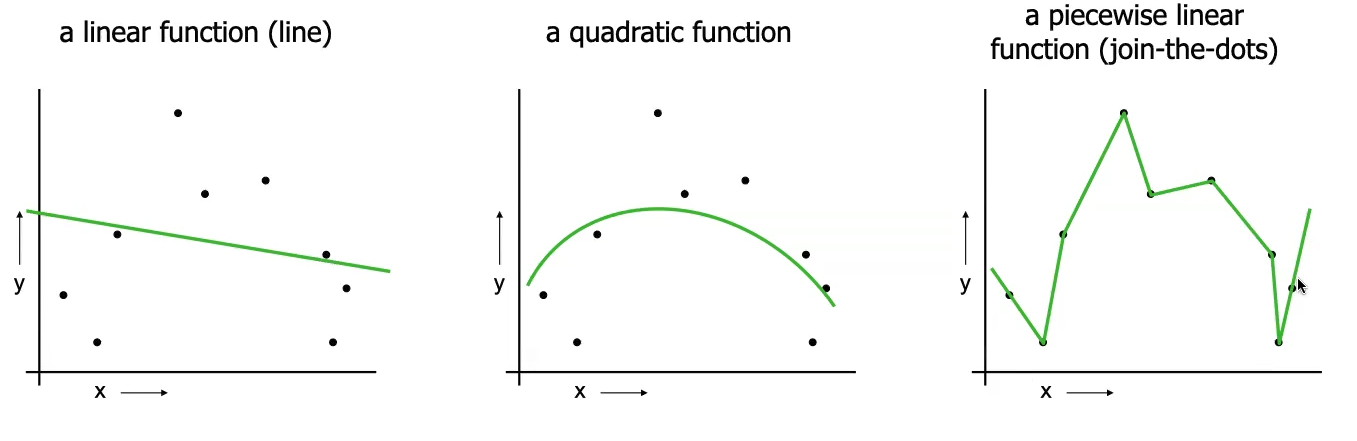
\includegraphics[scale=0.2]{screenshots/2026-03-11_3.png}
    \end{center}
	\begin{subparag}{Advantages}
	    \begin{itemize}
			\item Very simple
			\item We can choose the model based on the validation error
	    \end{itemize}
	\end{subparag}
\end{parag}
\begin{parag}{Leave-one-out cross-validation (LOOCV)}
	As an alternative method for the validation set method, we can use \important{LOOCV}: we will take one sample at a time and treat it as a validation sample, and we will loop through each sample as a validation sample. \\
	$ $\\
	For $i =  1, \ldots, N$
	\begin{enumerate}
		\item Let $\left(x_i ,y_i\right)$ be the i$\Th$ sample 
		\item Temporarily remove $\left(x_i, y_i\right)$ from the training set
		\item Perform regression on the remaining $N - 1$ samples 
		\item Compute the error on $\left(x_i, y_i\right)$
	\end{enumerate}
    \begin{center}
    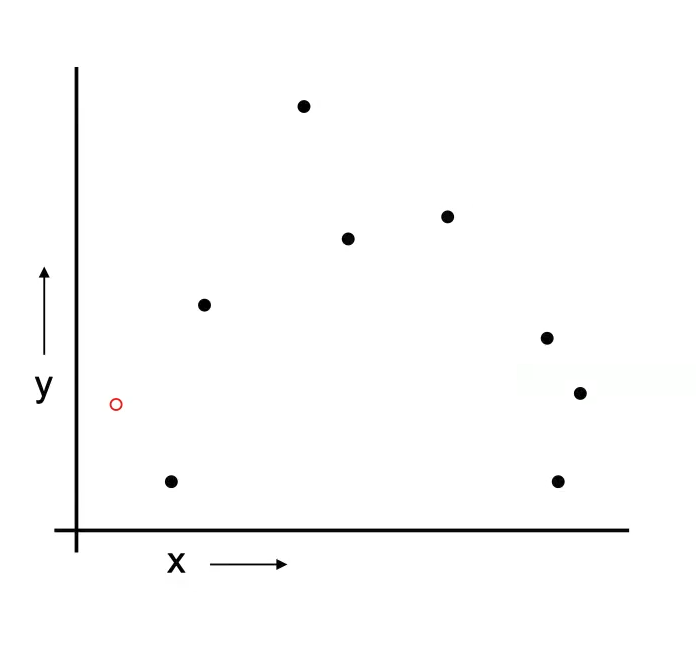
\includegraphics[scale=0.2]{screenshots/2026-03-24.png}
    \end{center}
	When you have done all points, report the average error. So if we take our 9 samples and we therfore fit 9 models, one for each points, we get the following curve (for a linear model) 
	\begin{center}
	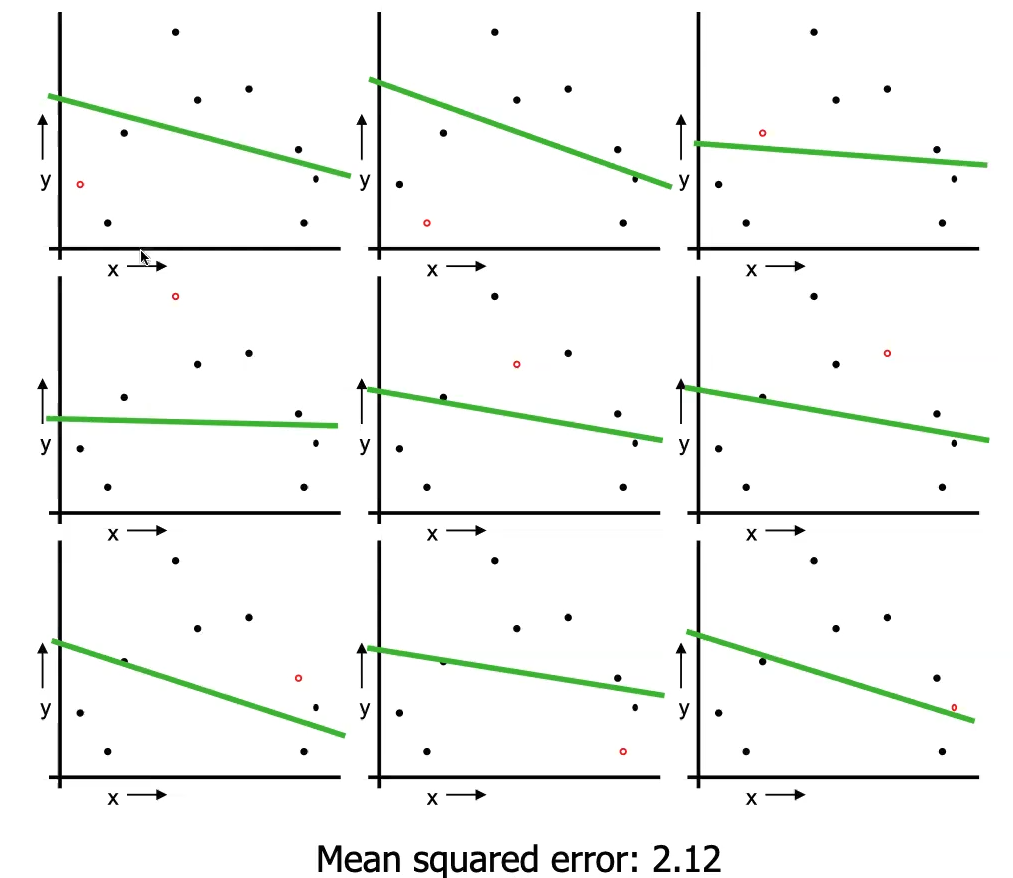
\includegraphics[scale=0.2]{screenshots/2026-03-24_1.png}
	\end{center}
	For each of those model we have \important{one} test data which will gives us an error, given the average error for all models, we have $2.12$. \\
	$ $\\
	But is this the best model? Now we can check and be pretty sure about our metriics. For instance, let us use a squared model:
	\begin{center}
	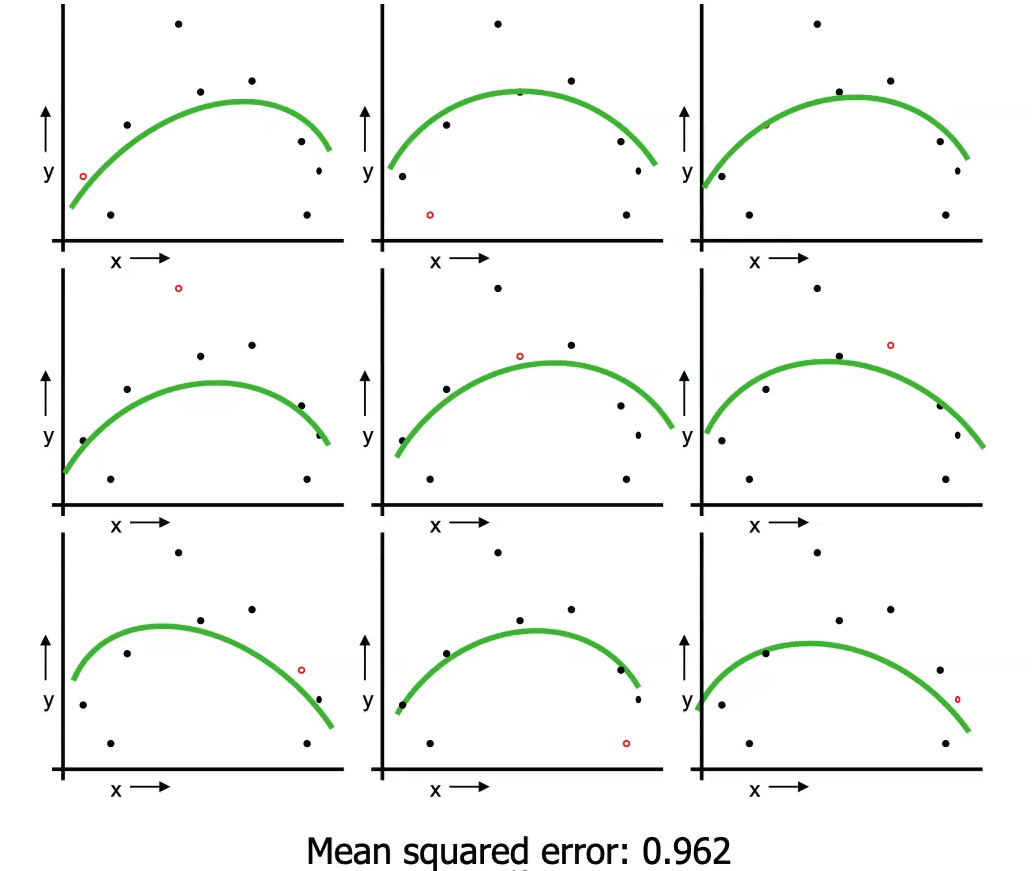
\includegraphics[scale=0.2]{screenshots/2026-03-24_2.png}
	\end{center}
	So as we can see, this type of cross-validation is pretty expensive, we have to train $N$ times for \important{each model}! So which one is best?

\end{parag}

\begin{center}
\begin{tabular}{|c|c|c|}
	\hline
	& Downside & Upside \\
	\hline
	\hline
	Validation-set & Unreliable estimate of future performance & Cheap  \\
	\hline
	Leave-one-out & Expensive & Doesn't waste data \\
	\hline
\end{tabular}
\end{center}

Both are a bit extreme, let us now look for something that is lying in the middle, \important{$k$-fold cross-validation}. First recall what were the issue about our two previous methods. The first one was that everything was fixed, the size of the test, the data that we used for training \important{and} for testing. The result of this is that the prediction of the future performance is unreliable (we could just be lucky with our test data). The issue with the second methods was that it was too expensive to compute because we needed to  compute a new model \important{for each point}. But why each point, why don't we just randomly split the data set into $k$ partitions (e.g., $k = 3$, shown with the different colors)
\begin{center}
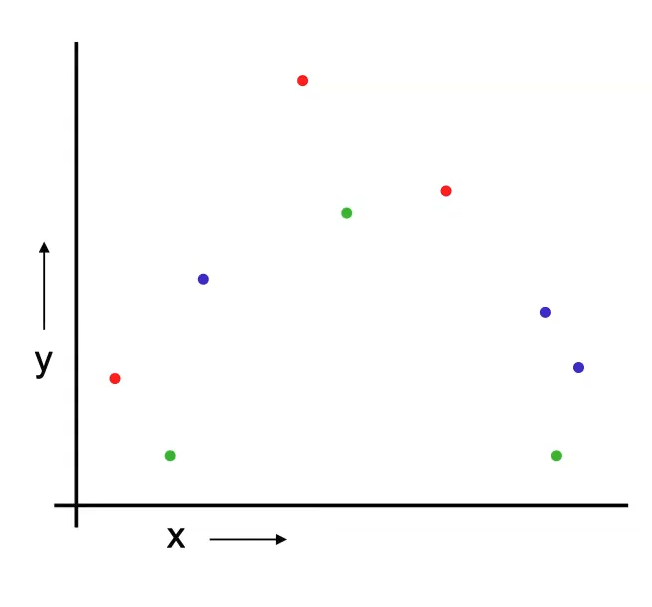
\includegraphics[scale=0.3]{screenshots/2026-03-24_3.png}
\end{center}
And now we do the same thing as what we did before but on partitions: we iterate through our partitions, we train our data in $\left\{\text{data set}\right\}\setminus \left\{\text{partitions}\right\}_i$. Then we compute the errors on the partitions$_i$. We then report the average error on all points.


\begin{center}
	\begin{tabular}{|c|p{6cm}|p{6cm}|}
	\hline
	& Downside & Upside \\
	\hline
	\hline
	Validation-set & Unreliable estimate of future performance & Cheap  \\
	\hline
	Leave-one-out & Expensive & Doesn't waste data \\
	\hline
	10-fold & Wastes 10\% of the data. 10 times more expensive than Validation-set & Only wastes \%. Only 10 times more expensive instead of $N$ \\
	\hline
	3-fold & Wastier than $10$-fold. Expensivier than validation-set & Slightly better than validation set \\
	\hline
	$N$-fold & Identival to Leave-one-out&&\\
	\hline
\end{tabular}
\end{center}

\begin{framedremark}
When we say "\textit{Wastes 10\%}" this doesn't mean that there is litteraly 10\% of the data that go to the trash bin, what this means is that when \important{evaluating} the performance of our model, we loose does 10\% for each fold. But not in the final training nor  in the overall process of the cross-validation.
\end{framedremark}
But ultimately there is not a best validation method. In practice one usually don't use Leave-one-out as it is too expensive. The $k$-fold is quite common when the model is not to expensive to train, but in the context of deep neural networks, almost everyone uses validation set.


\begin{parag}{Cross-validation}
    Cross-validation can help to:
	\begin{itemize}
		\item Select the best model among a small number of candidates
		\item Find the best value for one hyper-parameter (e.g. $k$ in k-NN)
			\begin{itemize}
				\item For this, one treats each value of the hyper-parameter as a separate model
			\end{itemize}
	\end{itemize}
	However, it becomes impractival with too many candidates, for example, one cannot choose which combination of functions to use for features expansion among a very large set.
\end{parag}


Now we have one tool in order to have a model that can generalize well. Let us now look at another way to prevent overfitting by penalizing model complexity via \important{regularization}. But before that let us go back to linear model.


\begin{parag}{Overfitting with a linear model}
    Because the linear model is simple, overfitting occurs fairly rarely. Nevertheless, if there are fewer training samples than input dimensions ($N \leq D  + 1$), then one can alwazs fit a hyperplan that passes exactly through the training samples.
	\begin{subparag}{Proof}
	    This can easily been check $N$ points in $D + 1$ dimensions. Our linear model will be given as $w^{T}x + b$. Let us simplify notation by absorbing the bias into the vector $\widetilde{x} = \left(x_1, \ldots, x_D, 1\right)$ then $\widetilde{w} \in \mathbb{R}^{D + 1}$ and our model $f$ is given as:
		\begin{align*} 
			f\left(x\right) = \widetilde{w}^{T}\widetilde{x}
		\end{align*}
		The input dimensions is $D + 1$ and the parameter vector is $w \in \mathbb{R}^{D + 1}$. Given $N$ training samples:
		\begin{align*} 
			\left(x^{\left(1\right)}, y^{\left(1\right)}\right), \ldots, \left(x^{\left(N\right)}, y^{\left(N\right)}\right)
		\end{align*}
		After the augmentation with have that each $\widetilde{x}^{\left(i\right)} \in \mathbb{R}^{D + 1}$ Then what we atre saying is that we want our model to fit perfectly i.e.:
		\begin{align*} 
			w^{\left(T\right)}\widetilde{x}^{\left(i\right)} = y^{\left(i\right)}, \mathspace \forall i = 1, \ldots, N
		\end{align*}
		Now let us stack our vector $\widetilde{x}$ and defined $X \in \mathbb{R}^{N \times \left(D +1\right)}$, where each row is $\left(\widetilde{x}^{\left(i\right)}\right)^{T}$:
		\begin{align*} 
			X = \begin{pmatrix} - & \left(\widetilde{x}^{\left(1\right)}\right)^{T} & - \\ - & \left(\widetilde{x}^{\left(2\right)}\right)^{T} & - \\  & \vdots &  \\ - & \left(\widetilde{x}^{\left(N\right)}\right)^{T} & - \end{pmatrix} 
		\end{align*}
		This gives us the final system
		\begin{align*} 
			Xw = y
		\end{align*}
		This implies that we have a linear systems with $N$ equations and $D + 1$ unknows, this is solvable when $N \leq D + 1$
	\end{subparag}
\end{parag}

\begin{parag}{Penalizin overfitting}
    THe standard way to penalize the complexity of a model is to add a regularizer to the empirical risk. This leads to a new training objective function of the form:
	\begin{align*} 
		E\left(w\right) = R\left(w\right) + \lambda E_w\left(w\right)
	\end{align*}
	Where $R\left(w\right)$ is the empirical risk and $E_w\left(w\right)$ is the regulariyer. $\lambda$ is a hyper-parameter that defines the influence of the regularizer $\left(\lambda > 0\right)$
\end{parag}
\begin{parag}{Regulariyed linear regression}
    One of the most common regularizers is the sum of squares of the weights (there is a probabilistic motivation behind it)
	\begin{align*} 
		E_w\left(w\right) = w^{T}w
	\end{align*}
	This lets us write regulariyed linear regression as
	\begin{align*} 
		\min_w \sum_{i= 1}^{N}\left(\phi\left(x_i\right)^{T}w - y_i\right)^2 + \lambda w^{T}w
	\end{align*}
	This remains a convex function (for $\lambda \geq 0$) and so we can still find the solution by zeroing out the gradient. But if you insists to compute the gradient\ldots
	\begin{align*} 
		\nabla E &= \nabla R  + \nabla E_w\\
				 &= 2 \sum_{i = 1}^{N}\phi\left(x_i\right)\left(\phi\left(x_i\right)^{T}w - y_i\right) + 2\lambda w
	\end{align*}
	As we can see the only differences is the new $2\lambda w$, the other terms is the same as what we saw in earlier lectures.\\
	$ $\\
	Setting the gradient to zero yields
	\begin{align*} 
		\left(\sum_{i= 1}^{N}\phi\left(x_i\right)\phi\left(x_i\right)^{T} + \lambda I_F\right)w^{\ast} =  \sum_{i= 1}^{N}\phi\left(x_i\right)y_i
	\end{align*}
	\begin{subparag}{Solution}
	    ultimately if we group the inputs in a matrix $\Phi$ and the output in a vector $y$, as before, this gives us the final solution:
		\begin{align*} 
			w^{\ast} = \left(\Phi^{T}\Phi + \lambda I_F\right)^{-1} \Phi^{T}y
		\end{align*}
		This also ensures that we can actually find a solution, that the matrix (the thing inside the parenthesis) can be inverted.
	\end{subparag}
	\begin{subparag}{Remark}
	    For people who have done cs-328, this is the Tikhonov regulariyation technic that we have seen. In cs-328 the goal of regularization was to \important{improve the condition number} of a problem. The geometric interpretation was that the addition of an identiy matric causes the matrix to scale input vectors uniformly in different directions
		\begin{center}
		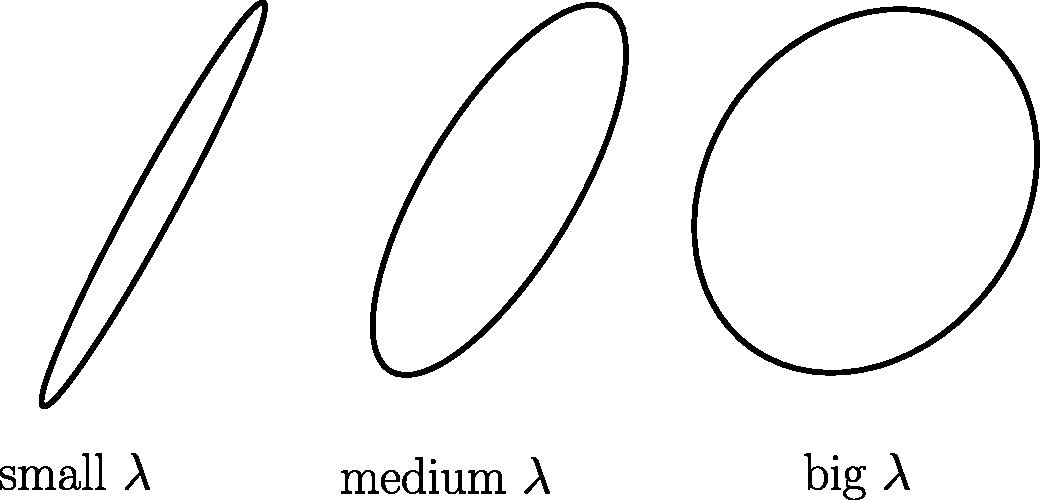
\includegraphics[width=0.8\textwidth]{figure/2026-03-24.pdf}
		\end{center}
		And this is the same thing as what we said above, the goal here is to improve the condition number $\implies$ having a matrix that is numericaly stable, that can be inverted
	\end{subparag}
	Note that the regularizer affects the optimal value of the parameters, but not the mathematical form of the prediction which remains the same.

\end{parag}
\begin{parag}{Multi-output ridge regression}
    When dealing with multiple output dimesnions, the parameters are expressed in matrix form. We can write multi-output ridge regression as:
	\begin{align*} \min_W \sum_{i= 1}^{N}\left\|W^{T}\phi\left(x_i\right)-y_i\right\|^2 + \lambda \left\|W\right\|_F^2 \end{align*}
	Where $\left\|W\right\|_F^2$ is the square Frobenius norm, equivalent to the sum of the square of all values in the matrix $W$.\\
	$ $\\
	By zeroing out the gradient, we obtain the solution:
	\begin{align*} 
		W^{\ast} = \left(\Phi^{T}\Phi + \lambda I_F\right)^{-1} \Phi^{T}Y
	\end{align*}
\end{parag}



\begin{parag}{Regularization and logistic regression}
    Regularization may also be added to the cross-entropy loss used to train the logistic regression model.
	\begin{itemize}
	    \item With a convex regularizer, such as the sum of squares, the overall regularized risk remains convex
	    \item The scikit-learn implementation of logistic regression has such an $L^2$ regularizer by default
	\end{itemize}
	
\end{parag}

\begin{parag}{Finding the right regularization strength}
    Note that the use of a regularizer leads to another hyper-parameter for the model, $\lambda$. And this parameter cannot be optimize, (the solution for it is $\lambda = 0$ which is not what we wanted and the reason on why we have introduced it in the first place). But if we cannot optimize it, how should we set its value? IDK
\end{parag}








